%% =====================================================================
%%  CRYSTAL -- ACM Transactions on Multimedia Computing, Communications,
%%  and Applications (TOMM) manuscript
%%
%%  Build: pdflatex -> bibtex -> pdflatex -> pdflatex  (Overleaf default)
%%
%%  MODE SWITCH -- pick ONE of the two lines below:
%%    review,anonymous  : double-anonymous submission PDF (line numbers,
%%                        authors hidden, "our prior work" must be 3rd person)
%%    (none)            : camera-ready / author preprint
%% =====================================================================
\documentclass[acmsmall,review,anonymous,screen]{acmart}
%\documentclass[acmsmall,screen]{acmart}

%% ------------------------------------------------------------------
%% ACM journal metadata (fill in after acceptance; harmless while blank)
%% ------------------------------------------------------------------
\acmJournal{TOMM}
\acmYear{2026}
\acmVolume{0}
\acmNumber{0}
\acmArticle{0}
\acmMonth{0}
\acmDOI{XXXXXXX.XXXXXXX}
\copyrightyear{2026}
\setcopyright{acmlicensed}

%% ------------------------------------------------------------------
%% Packages -- acmart already loads amsmath, amssymb, graphicx,
%% hyperref, booktabs, natbib, xcolor, microtype, caption, subcaption?
%% (subcaption is NOT loaded; added below)
%% ------------------------------------------------------------------
\usepackage{subcaption}
\usepackage{siunitx}
\usepackage{pgfplots}
\pgfplotsset{compat=1.18}
\usepgfplotslibrary{groupplots}
\usepackage{tikz}
\usetikzlibrary{arrows.meta,positioning,shapes.geometric,calc,fit,backgrounds}
\usepackage{multirow}
\usepackage{tabularx}
\usepackage{makecell}
\usepackage{pifont}
% Positioning-table symbols (MOSAIC/VQUEST style)
\newcommand{\yes}{\textcolor{green!60!black}{\ding{51}}}
\newcommand{\no}{\textcolor{red!80!black}{\ding{55}}}
\newcommand{\partially}{$\sim$}
\renewcommand{\theadfont}{\bfseries\footnotesize}
\usepackage{algorithm}
\usepackage{algpseudocode}
\usepackage{xspace}
\usepackage[inline]{enumitem}
\usepackage{orcidlink}
\usepackage[acronym,nomain,nopostdot,nogroupskip,nohypertypes={acronym},toc=false]{glossaries}
\glsdisablehyper
%% =====================================================================
%%  Acronyms (glossaries package). First use via \gls{} prints
%%  "long (SHORT)"; later uses print SHORT. Plural: \glspl{}.
%%  Force forms: \glsentryshort{}, \glsentrylong{}, \acrshort{}.
%%  Corrections vs. the qualification list are marked %% FIXED.
%% =====================================================================

%% --- Networks and generations ---
\newacronym{5g}{5G}{fifth-generation mobile networks}
\newacronym{6g}{6G}{sixth-generation mobile networks}
\newacronym{p5g}{P5G}{private 5G}
\newacronym{sa}{SA}{standalone}
\newacronym{ran}{RAN}{radio access network}
\newacronym{urllc}{URLLC}{ultra-reliable low-latency communications}
\newacronym{embb}{eMBB}{enhanced mobile broadband}
\newacronym{mmtc}{mMTC}{massive machine-type communications}
\newacronym{kpi}{KPI}{key performance indicator}
\newacronym{nfv}{NFV}{network function virtualization}
\newacronym{sdn}{SDN}{software-defined networking}      %% FIXED: "Software Defined Network" -> SDN is the paradigm, not a network
\newacronym{p4}{P4}{Programming Protocol-independent Packet Processors}
\newacronym{p7}{P7}{P4 Programmable Patch Panel}
\newacronym{bmv2}{bmv2}{behavioral model version 2}
\newacronym{du}{DU}{distributed unit}                    %% FIXED: singular

%% --- Transport ---
\newacronym{tcp}{TCP}{Transmission Control Protocol}      %% FIXED: short form was "TCP-HTTP"
\newacronym{udp}{UDP}{User Datagram Protocol}
%% QUIC: RFC 9000 states it is a name, not an acronym -> written literally via \quic, no entry
\newacronym{http3}{HTTP/3}{Hypertext Transfer Protocol version 3}
\newacronym{webrtc}{WebRTC}{Web Real-Time Communication}
\newacronym{dash}{DASH}{Dynamic Adaptive Streaming over HTTP}
\newacronym{hol}{HOL}{head-of-line}                      %% FIXED: "Head of Line Block" -> used as "\gls{hol} blocking"
\newacronym{rtt}{RTT}{round-trip time}
\newacronym{pto}{PTO}{probe timeout}
\newacronym{tls}{TLS}{Transport Layer Security}
\newacronym{cdn}{CDN}{content delivery network}
\newacronym{gcc}{GCC}{Google Congestion Control}
\newacronym{tc}{TC}{Linux Traffic Control}
\newacronym{w3c}{W3C}{World Wide Web Consortium}
\newacronym{ietf}{IETF}{Internet Engineering Task Force}

%% --- Immersive media ---
\newacronym{vr}{VR}{virtual reality}
\newacronym{ar}{AR}{augmented reality}
\newacronym{xr}{XR}{extended reality}
\newacronym{mxr}{MXR}{multisensorial extended reality}
\newacronym{6dof}{6DoF}{six degrees of freedom}
\newacronym{hmd}{HMD}{head-mounted display}              %% FIXED: hyphenated, lower case
\newacronym{fov}{FoV}{field of view}
\newacronym{fps}{fps}{frames per second}                 %% FIXED: unit is conventionally lower case
\newacronym{3dgs}{3DGS}{3D Gaussian Splatting}

%% --- Point clouds and coding ---
\newacronym{mpeg}{MPEG}{Moving Picture Experts Group}
\newacronym{pc}{PC}{point cloud}
\newacronym{pcc}{PCC}{point cloud compression}
\newacronym{vpcc}{V-PCC}{Video-based Point Cloud Compression}
\newacronym{gpcc}{G-PCC}{Geometry-based Point Cloud Compression}
\newacronym{v3c}{V3C}{Visual Volumetric Video-based Coding}
\newacronym{gof}{GOF}{group of frames}
\newacronym{hevc}{HEVC}{High Efficiency Video Coding}
\newacronym{hm}{HM}{HEVC Test Model}
\newacronym{tmc2}{TMC2}{Test Model Category 2}
\newacronym{ctc}{CTC}{common test conditions}
\newacronym{ra}{RA}{random access}
\newacronym{ldp}{LDP}{low-delay P}
\newacronym{qp}{QP}{quantization parameter}
\newacronym{lf}{LF}{light field}

%% --- Quality assessment ---
\newacronym{qoe}{QoE}{quality of experience}
\newacronym{qos}{QoS}{quality of service}
\newacronym{mos}{MOS}{mean opinion score}                %% FIXED: singular
\newacronym{acr}{ACR}{absolute category rating}           %% FIXED: key acr was ACR-HR; split
\newacronym{acrhr}{ACR-HR}{absolute category rating with hidden reference}
\newacronym{dsis}{DSIS}{double-stimulus impairment scale}
\newacronym{dscqs}{DSCQS}{double-stimulus continuous quality scale}
\newacronym{dcr}{DCR}{degradation category rating}
\newacronym{itu}{ITU}{International Telecommunication Union}
\newacronym{psnr}{PSNR}{peak signal-to-noise ratio}
\newacronym{vmaf}{VMAF}{Video Multimethod Assessment Fusion}
\newacronym{pcqm}{PCQM}{Point Cloud Quality Metric}
\newacronym{ssim}{SSIM}{structural similarity index}
\newacronym{fr}{FR}{full-reference}
\newacronym{rr}{RR}{reduced-reference}
\newacronym{nr}{NR}{no-reference}

%% --- Statistics ---
\newacronym{ci}{CI}{confidence interval}
\newacronym{clmm}{CLMM}{cumulative link mixed model}
\newacronym{plcc}{PLCC}{Pearson linear correlation coefficient}
\newacronym{srocc}{SROCC}{Spearman rank-order correlation coefficient}
\newacronym{rmse}{RMSE}{root mean square error}

\makenoidxglossaries

\graphicspath{{figures/}}
\sisetup{detect-all,per-mode=symbol,range-phrase=--,range-units=single}

%% ------------------------------------------------------------------
%% Macros: keep terminology consistent across the whole manuscript.
%% Acronyms route through glossaries, so first use expands automatically.
%% ------------------------------------------------------------------
\newcommand{\crystal}{\textsc{Crystal}\xspace}
\newcommand{\mosaic}{\textsc{Mosaic}\xspace}
\newcommand{\vquest}{\textsc{Vquest}\xspace}
\newcommand{\vpcc}{\gls{vpcc}\xspace}
\newcommand{\gpcc}{\gls{gpcc}\xspace}
\newcommand{\quic}{QUIC\xspace}   % RFC 9000: a name, not an acronym
\newcommand{\pcqm}{\gls{pcqm}\xspace}
\newcommand{\qoe}{\gls{qoe}\xspace}
\newcommand{\mos}{\gls{mos}\xspace}
\newcommand{\hmd}{\gls{hmd}\xspace}
\newcommand{\gof}{\gls{gof}\xspace}
\newcommand{\gofs}{\glspl{gof}\xspace}
\newcommand{\fiveg}{\gls{5g}\xspace}
\newcommand{\threedgs}{\gls{3dgs}\xspace}
\newcommand{\plr}{\mathrm{PLR}}
\newcommand{\tlf}{\psi}                      % skip fraction
\newcommand{\qc}{\widetilde{Q}_c}            % per-content clean ceiling
% Math-safe short forms (glossaries inside math is fragile)
\newcommand{\mosm}{\mathrm{MOS}}

% The CRYSTAL model, in one place (edit here, propagate everywhere)
% Layer 2 (perceptual): one free parameter alpha, per-content ceiling Qc
\newcommand{\crystalmodel}{%
  \widehat{\mosm} = 1 + 4\,\qc\, e^{-\alpha \tlf}}
% Layer 1 (transport): skip fraction from session counters
\newcommand{\crystallayerone}{%
  \tlf = \frac{\text{units skipped} + \text{units jumped over}}{\text{units due}}}

% Online Appendix switch: \appendixfalse hides it (body page count only);
% the appendix cross-references in Section 4 are wrapped in \ifappendix.
\newif\ifappendix
\appendixfalse

% Editorial helpers (remove before submission)
\newcommand{\todo}[1]{\textcolor{red}{[TODO: #1]}}
\newcommand{\note}[1]{\textcolor{blue}{[NOTE: #1]}}

% Anonymisation. acmart provides \anon[review]{final}, which paints the
% review text orange -- good for short placeholders. For whole
% paragraphs that must read naturally in both modes, use \blind:
\makeatletter
\newcommand{\blind}[2]{\if@ACM@anonymous #1\else #2\fi}
\makeatother

%% ------------------------------------------------------------------
%% Title / authors
%% ------------------------------------------------------------------
\title[CRYSTAL: A Mechanistic QoE Model for V-PCC over Reliable QUIC]{%
  \crystal: A Mechanistic Two-Layer Quality-of-Experience Model for
  V-PCC Volumetric Video Streaming over Reliable QUIC on Private 5G}

\author{Alan Teixeira da Silva}
\orcid{0000-0000-0000-0000}
\email{a.silva@unicamp.br}
\affiliation{%
  \institution{School of Electrical and Computer Engineering (FEEC), University of Campinas (UNICAMP)}
  \city{Campinas}
  \state{SP}
  \country{Brazil}}

\author{Vanessa Testoni}
\orcid{0000-0000-0000-0000}
\email{vanessa@unicamp.br}
\affiliation{%
  \institution{FEEC, University of Campinas (UNICAMP)}
  \city{Campinas}
  \state{SP}
  \country{Brazil}}

\author{Christian Esteve Rothenberg}
\orcid{0000-0000-0000-0000}
\email{chesteve@unicamp.br}
\affiliation{%
  \institution{FEEC, University of Campinas (UNICAMP)}
  \city{Campinas}
  \state{SP}
  \country{Brazil}}

\renewcommand{\shortauthors}{Teixeira da Silva et al.}

%% ------------------------------------------------------------------
%% Abstract (structured: problem, gap, approach, result, claim)
%% ------------------------------------------------------------------
\begin{abstract}
Volumetric video for virtual reality is delivered to the edge over the
\quic that production stacks ship, which is fully reliable: a lost
packet never corrupts the decoded point cloud, it delays it. Under
\gls{mpeg} \vpcc, whose bitstream is organized in groups of frames
that must arrive in full before a presentation deadline, delay and
loss therefore reach the viewer only as freezes and skips. Existing
network-aware \qoe models for volumetric media fit delay and loss
directly, with coefficients re-estimated per quality level, and
generalize poorly. We present \crystal, a two-layer model in which the
transport layer has no perceptual parameter and the perceptual layer
has one. Layer~1 explains how delay and loss turn into skipped
delivery units through a per-unit budget, a slack that delay shrinks
and each loss spends, and a decoder buffer that drains when slow
units run in sequence; it predicts the pure-delay threshold without
a fitted parameter and shows that delay and loss cannot act
separably. Layer~2 maps the measured skip fraction $\tlf$ to opinion
score as $\crystalmodel$, with the ceiling $\qc$ read from the clean
condition. We also document the end-to-end pipeline on which the
model is tested, extending our conference paper: a shim that makes
reference \vpcc encoding tractable, a native \gls{http3} client and
deadline scheduler feeding the 5G-MAG decoder, a direct OpenVR
presentation path, a 5G-capable Meta Quest~3, and an impairment chain
cleared of six transport confounds. An ITU-T P.910 study
($N=50$) over four impairment slices at a fixed encoder tests whether
ratings depend on the network only through presentation timing.
\todo{Results.}
\end{abstract}

%% ------------------------------------------------------------------
%% CCS concepts -- generate at https://dl.acm.org/ccs and paste
%% ------------------------------------------------------------------
\begin{CCSXML}
<ccs2012>
   <concept>
       <concept_id>10002951.10003227.10003251.10003256</concept_id>
       <concept_desc>Information systems~Multimedia streaming</concept_desc>
       <concept_significance>500</concept_significance>
   </concept>
   <concept>
       <concept_id>10003120.10003121.10003124.10010870</concept_id>
       <concept_desc>Human-centered computing~Virtual reality</concept_desc>
       <concept_significance>300</concept_significance>
   </concept>
   <concept>
       <concept_id>10003033.10003079.10011704</concept_id>
       <concept_desc>Networks~Network measurement</concept_desc>
       <concept_significance>300</concept_significance>
   </concept>
</ccs2012>
\end{CCSXML}
\ccsdesc[500]{Information systems~Multimedia streaming}
\ccsdesc[300]{Human-centered computing~Virtual reality}
\ccsdesc[300]{Networks~Network measurement}

\keywords{volumetric video, point cloud streaming, quality of experience,
V-PCC, QUIC, HTTP/3, private 5G, subjective assessment, virtual reality}

%% ------------------------------------------------------------------
\begin{document}
\maketitle
\glsresetall

\section{Introduction}
\label{sec:intro}

Immersive applications increasingly define the trajectory from \fiveg
to \gls{6g}~\cite{liberg2024,shen2023toward}: 3GPP and ITU-R list
immersive and extended-reality services among the primary usage
scenarios of these generations~\cite{3gpp22261,itur-m2160}, and mobile
video traffic is projected to more than double by
2031~\cite{mobility25nov}. The most demanding of these services is
immersive media streaming for \gls{vr}: volumetric content captured from
a real scene and reproduced in an \gls{hmd} with
\gls{6dof}~\cite{Immersivevideo,Viola2023}. Its dominant format, the
dynamic point cloud, requires gigabits per second
uncompressed~\cite{pcstreaming21}, and \gls{mpeg}'s
\gls{vpcc}~\cite{v3c,vpccgraziosi} is the reference codec for dense,
dynamic content. \vpcc codes geometry, attribute and occupancy atlases
with \gls{hevc}~\cite{hevc} and inherits its temporal prediction
structure: the bitstream is organised in \glspl{gof}, each of which must
be received in full before any of its frames can be decoded. Because
standalone \glspl{hmd} cannot decode \vpcc in real time, deployments
render at an edge server and cast the frames to the headset, so the
path from the content origin to the edge renderer is where network
impairment reaches the content.

Volumetric streaming research has largely assumed lossy datagram
transport or partially reliable \quic variants that drop stale
data~\cite{ravuri2023,haseeb2025}. Production systems run neither: the
\quic shipped in browsers, content delivery networks and mobile
operating systems is fully reliable~\cite{rfc9000}. No bitstream reaches
the decoder incomplete; loss becomes delay through retransmission and
congestion-window reduction, and the \gof amplifies that delay, since
one late packet stalls the whole unit. The perceptual consequence is
temporal rather than geometric: freezes and frame skips, not holes in
the surface. Our earlier work showed that latency and loss leave
distinct transport signatures~\cite{vquest2026}, and that a \vpcc slice
with \emph{lower} loss but a tighter \gof deadline can score lower
than one with higher loss~\cite{mosaic2026}. Existing \qoe models do not
capture this regime. The closest, by Udora et
al.~\cite{qoeholographic,udora2026tmm}, fits an exponential-in-delay,
linear-in-loss regression per quality level and reaches held-out
correlations of 0.57--0.66; it describes its data but not \emph{why}
delay and loss degrade \qoe, and so cannot transfer to a new \gof size,
encoder or network. Subjective \vpcc studies, meanwhile, inject loss
offline or assess outside fully occlusive
\gls{vr}~\cite{dumic2023,nguyen2023,Cox2023}.

We present \crystal, a mechanistic two-layer \qoe model for \vpcc
streaming over reliable \quic. Layer~1, which has no perceptual
parameter, derives the \emph{temporal loss fraction} $\tlf$, the fraction
of wall-clock time in which the renderer has no fresh \gof to show, from
delivery slack, round-trip time, loss-recovery cost and \gof size.
Layer~2 maps $\tlf$ to opinion score with one constant,
\begin{equation}
  \crystalmodel,
  \label{eq:crystal-intro}
\end{equation}
where $\qc$ is the clean-reference ceiling of each content and $\alpha$
is the only fitted parameter. The model claims that, under reliable
transport, latency and loss act on \qoe only through $\tlf$. We test it
with an ITU-T P.910 \gls{acr} study ($N=50$) on a private \fiveg testbed
that streams \vpcc over \gls{http3} to an edge renderer and casts the
rendered frames to Meta Quest~3 headsets, using a $2\times2$ factorial
design that separates latency, loss and their interaction at a fixed
encoder configuration. The contributions are:
\begin{enumerate}[leftmargin=*,nosep]
  \item \textbf{A mechanistic model} whose transport layer is
        parameter-free and whose perceptual layer has one constant,
        replacing per-quality-level regression coefficients with a
        single explanatory variable, $\tlf$.
  \item \textbf{A pre-registered factorial evaluation} showing that
        latency and loss each degrade perceived smoothness and together
        degrade it $1.61\times$ more than the sum of the two, refuting
        the additivity of prior regressions; that \gof structure rather
        than loss magnitude governs resilience, a larger low-delay \gof
        being more robust than a smaller one; and that a single
        $\alpha$ \todo{does / does not} predict held-out conditions.
  \item \textbf{A transport characterisation and dataset}: per-\gof
        stall and deadline-miss measurements of reliable \quic under
        controlled impairment, and \todo{$N$} ratings over three
        \gls{mpeg} test sequences collected in \gls{vr} with a
        reproducible rating application.
\end{enumerate}

\blind{%
This article extends two conference papers: \cite{mosaic2026}
introduced the \vpcc-over-\quic pipeline and a three-tier study
($N=20$) that paired impairment with encoder configuration, and
\cite{vquest2026} characterised the transport signatures of latency and
loss for a frame-independent codec; earlier testbed descriptions
appeared as demonstrations~\cite{bestdemo25,nfvsdn24}. Neither proposed
a model or isolated \gof structure.%
}{%
This article extends two conference papers by the authors:
\mosaic~\cite{mosaic2026} introduced the \vpcc-over-\quic pipeline and
a three-tier study ($N=20$) that paired impairment with encoder
configuration, and \vquest~\cite{vquest2026} characterised the
transport signatures of latency and loss for a frame-independent codec;
earlier testbed descriptions appeared as
demonstrations~\cite{bestdemo25,nfvsdn24}. Neither proposed a model or
isolated \gof structure.%
}
Section~\ref{sec:related} reviews related work,
Section~\ref{sec:model} derives the model and its predictions,
Section~\ref{sec:system} describes the testbed and experimental design,
Section~\ref{sec:results} reports the results,
Section~\ref{sec:discussion} discusses implications and limitations,
and Section~\ref{sec:conclusion} concludes.

\section{Related Work}
\label{sec:related}

This section reviews the literature on the components of the pipeline
in Figure~\ref{fig:architecture} and on the modelling problem this
article addresses: volumetric video delivery and the transports
proposed for it, subjective assessment of point-cloud video and of
temporal smoothness, and parametric \gls{qoe} models. The literature
was assembled in three passes: a seed set from the bibliographies of
the two conference studies this article extends and of the tutorial by
van der Hooft et al.~\cite{Immersivevideo}, followed by backward
snowballing; the identification of the closest prior model, Udora et
al.~\cite{qoeholographic,udora2026tmm}, and an examination of the works
citing it; and keyword searches of IEEE Xplore, the ACM Digital Library
and Google Scholar for 2023--2026 publications on the same topics.
Only peer-reviewed publications and standards were retained.
Table~\ref{tab:positioning} positions \crystal against the closest
studies.

\begin{table}[!t]
  \caption{Positioning of \crystal against related work.
  \yes{} = supported, \no{} = not addressed, \partially{} = partial.
  ``Network impairment'': delay and loss as controlled independent
  variables (\partially{} denotes bandwidth-only adaptation or offline
  loss injection); ``Reliable \quic'': unmodified, fully reliable \quic
  (\partially{} denotes reliable \gls{tcp} or a modified \quic);
  ``Mechanistic model'': the explanatory variable is derived from
  transport mechanics rather than fitted to delay and loss directly.}
  \label{tab:positioning}
  \centering
  \footnotesize
  \setlength{\tabcolsep}{3pt}
  \renewcommand{\arraystretch}{1.15}
  \begin{tabular*}{\textwidth}{@{\extracolsep{\fill}}llcccccc@{}}
    \toprule
    \thead[l]{Work} & \thead[l]{Codec} &
    \thead{Subjective\\Study} & \thead{VR\\Headset} &
    \thead{Network\\Impairment} & \thead{QoE\\Model} &
    \thead{Reliable\\\quic} & \thead{Mechanistic\\Model} \\
    \midrule
    van der Hooft et al.~\cite{vanderhooft2020qomex} & \vpcc  & \yes & \no        & \partially & \no  & \no        & \no \\
    Subramanyam et al.~\cite{subramanyam2022} & CWI-PCL    & \yes & \yes       & \partially & \no  & \no        & \no \\
    Cox et al.~\cite{Cox2023}               & \vpcc        & \yes & \no        & \no        & \no  & \no        & \no \\
    Nguyen et al.~\cite{nguyen2023}         & \vpcc        & \yes & \partially & \no        & \no  & \no        & \no \\
    Zhou et al.~\cite{zhou2025tomm}         & \vpcc, \glsentryshort{gpcc} & \yes & \yes       & \no        & \no  & \no        & \no \\
    Van Damme et al.~\cite{vandamme2024}    & \vpcc        & \yes & \no        & \no        & \yes & \no        & \no \\
    Dumic \& da Silva Cruz~\cite{dumic2023} & \vpcc        & \yes & \no        & \partially & \no  & \no        & \no \\
    Ravuri et al.~\cite{ravuri2023}         & \vpcc        & \no  & \no        & \yes       & \no  & \partially & \no \\
    Cetus~\cite{hou2026cetus}               & --           & \no  & \no        & \yes       & \no  & \partially & \no \\
    Sidhu \& Bentaleb~\cite{gpcc2026quic}   & \glsentryshort{gpcc}        & \no  & \no        & \partially & \no  & \yes       & \no \\
    Rudolph et al.~\cite{rudolph2025rabbit} & \vpcc        & \no  & \no        & \no        & \no  & \no        & \no \\
    Udora et al.~\cite{qoeholographic,udora2026tmm} & uncompressed & \yes & \yes & \yes & \yes & \partially & \no \\
    \mosaic~\cite{mosaic2026}               & \vpcc        & \yes & \yes       & \yes       & \no  & \yes       & \no \\
    \vquest~\cite{vquest2026}               & frame-indep. & \yes & \yes       & \yes       & \no  & \yes       & \no \\
    \midrule
    \textbf{\crystal (ours)}                & \vpcc        & \yes & \yes       & \yes       & \yes & \yes       & \yes \\
    \bottomrule
  \end{tabular*}
\end{table}

\subsection{Volumetric Video Delivery and Transport}
\label{sec:rw-systems}

Surveys of immersive media delivery describe the pipeline from capture
to \gls{6dof} rendering and identify \gls{qoe} under network impairment
as an open problem~\cite{Immersivevideo,Viola2023,shen2023toward};
Liu et al.~\cite{pcstreaming21} note that measuring the \gls{qoe} of point-cloud streaming is still in
its infancy, and Mozhganfar et al.~\cite{mozhganfar2026noms} classify
the \gls{qoe} models that do exist for volumetric streaming by input
factors and modelling strategy. The standards bodies have catalogued
the influence factors without modelling them: ITU-T
G.1035~\cite{itu_g1035} lists delay, bandwidth and loss among the
network factors and frame rate among the media factors that shape
\gls{vr} \gls{qoe}, and ITU-T P.1320~\cite{itu_p1320} extends the
catalogue to \gls{xr} meetings; neither maps those factors to a score
for volumetric content.

Streaming systems for \vpcc address bandwidth and adaptation. Rudolph
et al.~\cite{rudolph2025rabbit} transcode \vpcc streams in real time by
re-encoding only the video sub-streams; Shi et al.~\cite{qv424} add
viewpoint-aware tiling to \vpcc using the encoder's intermediate
outputs, with a \gls{qoe} model trained on VOLVQAD ratings.
Codec-agnostic systems exploit inter-frame correlation~\cite{hermes}
or neural super-resolution~\cite{yuzu}. These works evaluate with objective metrics or
simulation and hold the encoder configuration, in particular the \gof
length, fixed.

On the transport side, the dominant response to loss is to relax
reliability. Ravuri et al.~\cite{ravuri2023} integrate \gls{dash} with
partially reliable \quic for \vpcc, deciding per object whether to
deliver reliably, and report 46\% higher throughput and 33\% fewer
playout interruptions than reliable \quic at 5\% loss on 5G traces,
with a headless player. Haseeb et al.~\cite{haseeb2025} combine
adaptive encoding with a mixed-reliability \quic protocol; Freeman et
al.~\cite{moq2025} obtain implicit server-side adaptation from
Media-over-\quic delivery timeouts; and Hou et al.~\cite{hou2026cetus}
couple an application-level frame-drop policy to partially reliable
transmission for live volumetric video, reporting frame-rate and
objective-quality gains. A second response handles loss below the
transport: Qian et al.\ duplicate packets in eBPF between network nodes
so that volumetric frames meet their deadlines despite path
instability~\cite{qian2024ebpf}, and Thomas and
Xylomenos~\cite{thomas2025} stream point clouds with forward error
correction on a real 5G testbed without \quic. The one recent pipeline
that keeps production \quic unmodified, Sidhu and Bentaleb's
\gls{dash}-over-\quic delivery of \gpcc~\cite{gpcc2026quic}, finds that
\quic implementation choices materially affect delivery but evaluates
objectively, without a headset or a subjective study. Each of these
works modifies the fully reliable protocol that production stacks
ship~\cite{rfc9000}, handles loss outside it, or omits perceptual
evaluation; that reliable \quic turns loss into delay, and delay into
\gof stalls, is noted in several of them, but its perceptual cost has
not been quantified. Before~\cite{mosaic2026}, no study combined real
\vpcc transmission over \quic, playback in a \gls{vr} headset,
controlled impairment on a real link, 5G delivery and a standardised
subjective study, and no study yet combines those with a model.

\subsection{Subjective Quality Assessment}
\label{sec:rw-subjective}

Subjective studies of point-cloud video have concentrated on
compression and bandwidth. Van der Hooft et al.~\cite{vanderhooft2020qomex}
conduct the first subjective evaluation of adaptive \vpcc streaming,
with 30 participants rating pre-rendered viewports on a flat screen
under bandwidth and buffer variation at a fixed latency. Subramanyam
et al.~\cite{subramanyam2022} evaluate tiled user-adaptive streaming
for \gls{vr} remote communication with 33 users in head-mounted
displays, varying bandwidth. Cox et al.~\cite{Cox2023} release VOLVQAD,
7,680 ratings of 376 \vpcc sequences from 120 participants on 2D
displays, and find texture compression more damaging than geometry.
Nguyen et al.~\cite{nguyen2023} characterise \gls{qoe} and immersion of
\vpcc point clouds on the HoloLens~2 with 32 participants across
quantisation, quality switches, viewing distance and content. Zhou et
al.~\cite{zhou2025tomm} collect quality scores and eye-tracking maps
from 40 participants viewing \vpcc, \gpcc and CWI-PCL content with
\gls{6dof} in \gls{vr}. Alexiou et al.~\cite{Alexiou2023} review the
methodology; Ak et al.~\cite{ak2024basics} benchmark objective metrics
on a broad static corpus, where \pcqm~\cite{pcqm} is among the most
stable across codecs.

Few studies vary the network. Dumic and da Silva Cruz~\cite{dumic2023}
inject \SIrange{0.5}{2}{\percent} packet loss into \vpcc sub-bitstreams
before decoding and report \mos drops exceeding one scale unit at
\SI{0.5}{\percent}, with geometry and occupancy losses far more
damaging than attribute losses. Loss is applied to the bitstream
rather than produced by a transport, so the stimulus is
corruption rather than delay, and the content is shown as 2D video.
Our earlier study~\cite{mosaic2026} rated \vpcc in head-mounted
displays under real \quic impairment but paired each network tier with
a different encoder configuration, so the two factors could not be
separated. The only other subjective study under delay and loss on
reliable transport in head-mounted displays is that of Udora et al.,
discussed in Section~\ref{sec:rw-models}.

The attribute rated in this article is temporal smoothness, which has
a perceptual literature of its own outside point clouds. Judder on
head-mounted displays degrades the perceived quality of
omnidirectional video and interacts with compression
level~\cite{mahmoudpour2019judder}, and Klein et
al.~\cite{klein2024vft} show that frame-timing variations of about
\SI{12}{\milli\second} reduce perceived smoothness while variations of
about \SI{4}{\milli\second} barely do. These studies establish
smoothness as a ratable attribute distinct from fidelity; they do not
connect it to transport behaviour.

\subsection{\gls{qoe} Models}
\label{sec:rw-models}

Parametric \gls{qoe} models relate an impairment to a quality score.
The exponential form used in \crystal descends from the IQX hypothesis
of Fiedler et al.~\cite{fiedler2010}, which derives
$\mathrm{QoE} = a\,e^{-bx} + c$ for a single impairment $x$; Reichl et
al.~\cite{reichl2010} argue for a logarithmic law, and the two agree in
the operating region of interest~\cite{alreshoodi2013}. For buffered
video the impairment that matters is stalling: Ho{\ss}feld et
al.~\cite{hossfeld2011youtube} find an exponential dependence of \mos
on the number and length of stalling events, and the survey by Seufert et
al.~\cite{seufert2015survey} consolidates the stalling ratio as the
established temporal \gls{qoe} variable for HTTP streaming. ITU-T
P.1203~\cite{itu_p1203} standardises that view, folding initial delay,
rebuffering and quality switches into a session score. In all of these
the stalling term is \emph{measured} at the client; \crystal keeps the
exponential kernel and a stalling-type variable but \emph{derives} it
from transport mechanics, so that delay, loss and \gof length enter
only through it.

For volumetric media, three kinds of model have been proposed.
Streaming optimisers such as QV4~\cite{qv424} and Wang et
al.~\cite{wang2022tmm} embed a weighted sum of quality, quality
fluctuation and rebuffering as their objective; these are calibrated
on 2D-video conventions and evaluated in simulation, and Nguyen et
al.~\cite{qoedynamicpc} adapt P.1203 to dynamic point clouds in
\gls{ar} with the parameters of the 2D standard. Feature-based models
map content or device features to quality without a network variable:
Van Damme et al.~\cite{vandamme2024} train a
clustering-based psychometric model on no-reference image features for
\vpcc video at video, \gof and frame granularity, and Zhang et
al.~\cite{zhang2019towards} build a fuzzy inference system for the
HoloLens.

The third kind, and the closest to this work, is the network-aware
regression of Udora et al.~\cite{qoeholographic,udora2026tmm} for live
volumetric telepresence with uncompressed per-frame point clouds over
reliable \glsentryshort{tcp}. From a double-stimulus study with 25
participants in head-mounted displays they fit
\begin{equation}
  \mathrm{QoE} = a\,e^{b D} + c\,\plr + d,
  \label{eq:udora}
\end{equation}
with the coefficients re-estimated for each of three point-cloud
density levels and held-out \gls{plcc} of 0.57--0.66; the journal
version~\cite{udora2026tmm} embeds the model in a learning-based scheme
that adapts resolution and frame rate to user intent and network
state, and leaves \quic to future work. Two features make it the right
baseline. It is the only published model that predicts a subjective
score for volumetric content from network conditions under reliable
transport, so its data carry the same loss-to-delay signature that
\crystal sets out to explain; and its per-frame delivery is the
limiting case of no \gof coupling, which gives the \gof term of
\crystal an external reference point. \crystal differs in form (one
perceptual parameter instead of per-level coefficients), in
explanation (the delay--loss interaction is derived rather than
fitted, with its additive form treated as a prediction to be tested)
and in transport (production \quic rather than \glsentryshort{tcp}).

\section{The \crystal Model}
\label{sec:model}

\subsection{Scope and Rated Attribute}
\label{sec:model-scope}
\crystal models the \emph{network-attributable} component of \qoe for
\vpcc streaming over reliable \quic: the degradation in perceived
temporal smoothness caused by delay and loss, relative to an
impairment-free presentation of the same content. It does not model
compression fidelity, which is fixed per sequence and reported through
\pcqm as a stimulus descriptor, and it does not model overall \mos as a
combination of fidelity and smoothness. The rated attribute in the
subjective study is smoothness of playback. One quantity in the model
is fitted to ratings ($\alpha$), one is measured on the clean slice
($\qc$), and everything else is a transport fact, a client property or
a session counter (Table~\ref{tab:notation}).

\begin{table}[t]
  \caption{Notation. Values in parentheses are those of the campaign
  client of Section~\ref{sec:system}.}
  \label{tab:notation}
  \centering
  \footnotesize
  \setlength{\tabcolsep}{4pt}
  \begin{tabular}{@{}lll@{}}
    \toprule
    Symbol & Meaning & Source \\
    \midrule
    $G$, $F$ & \gof size (frames), frame rate & encoder \\
    $T_G = G/F$ & content-clock period of one delivery unit & derived (\SI{133.3}{\milli\second} at $G=4$) \\
    $f$ & client render-frame length & client, logged per session (\SI{30}{\milli\second}) \\
    $B_{\mathrm{eff}} = f(\lfloor T_G/f \rfloor - 1)$ & per-unit budget after frame quantization & derived (\SI{90}{\milli\second}) \\
    $d$ & added one-way delay & network condition \\
    $\tau_{\mathrm{dl}}$ & clean transfer time of a unit & pipeline log at $P=0$ ($\approx$35--\SI{39}{\milli\second}) \\
    $S(d) = B_{\mathrm{eff}} - \tau_{\mathrm{dl}} - d$ & slack: margin left for loss recovery & derived \\
    $P$ & packet loss rate & network condition \\
    $N_p$ & packets per unit & log ($\approx$471--517) \\
    $\mu = P N_p$ & expected losses per unit & derived \\
    $r(d) = r_0 + \kappa d$ & effective cost of one loss, incl.\ window cut & server transport logs \\
    $K(d) = \lfloor S(d)/r(d) \rfloor$ & losses a unit can absorb & derived \\
    $H$ & decoder lead over the content clock & client ($\approx$\SI{550}{\milli\second}, $\approx$4 units) \\
    $\tlf$ & skip fraction: (skipped + jumped) / due & session counters \\
    $\phi$ & freeze fraction: units shown late / due & session counters \\
    $\qc$ & clean-reference ceiling, $(\mosm_{A,c} - 1)/4$ & measured, Slice~A \\
    $\alpha$ & perceptual sensitivity to lost playout & fitted to ratings \\
    \bottomrule
  \end{tabular}
\end{table}

\subsection{Delivery Unit and Loss Recovery}
\label{sec:model-unit}
Two properties of the stream and the transport determine how a network
impairment reaches the viewer. The first is the delivery unit. \vpcc,
the principal component of ISO/IEC 23090-5~\cite{v3c,vpccgraziosi},
projects a dynamic point cloud into geometry, attribute and occupancy
atlases coded as ordinary video with \gls{hevc}~\cite{hevc,tmc2}, and so
inherits the video codec's prediction structure: frames are coded in
\glspl{gof}, either \gls{ra} with I-, P- and B-frames and a \gof of 32,
or \gls{ldp} with I- and P-frames and \gofs of 16 or
4~\cite{vpccctc,hmctc}. A \gof must be received in full before any of
its frames can be reconstructed, and in a streaming deployment it
carries a presentation deadline. The \gof is therefore the
\emph{delivery unit}, and its size sets the budget within which a
disturbance must be absorbed.

The second is loss recovery. Each \gof is fetched as one HTTP object
over \gls{http3}~\cite{rfc9114} on one \quic stream~\cite{rfc9000}.
\quic declares a packet lost either when a packet at least
$k_{\mathrm{PacketThreshold}}=3$ later is acknowledged or, if no later
acknowledgment arrives, when a \gls{pto} expires~\cite{rfc9002}:
\begin{equation}
  \mathrm{PTO} = \mathrm{sRTT} + \max(4\,\mathrm{RTT}_{\mathrm{var}},
  k_{\mathrm{granularity}}) + \mathrm{max\_ack\_delay}.
  \label{eq:pto}
\end{equation}
A loss therefore costs at least one round trip, and each recovery is
followed by a congestion-window reduction that persists into later
transfers. Because \quic is reliable, the decoder never receives an
incomplete \gof: loss becomes \emph{delay}, and delay becomes a
\emph{freeze} or a \emph{skip} when the unit misses its presentation
time. Our measurements show the two impairments leave distinct
signatures, added latency shifting the delivery-time distribution and
loss expanding its tail~\cite{vquest2026}, and that the per-\gof
deadline-miss rate correlates only partially with subjective quality
($\rho = -0.34$) because a missed \gof of 4 frames and one of 16
frames remove different durations of content~\cite{mosaic2026}.

\subsection{Layer 1: One Perceptual Channel}
\label{sec:model-layer1}

\subsubsection{Premises and claim}
Layer~1 rests on two premises. Under \emph{reliable transport}, a lost
packet never corrupts a decoded unit; it delays the unit's arrival.
Under \emph{deadline-enforced buffered playout}
(Section~\ref{sec:sys-edge}), the client keeps one request in flight
and feeds a decoder that holds about $H$ of content ahead of the
content clock; each unit has a fixed presentation time, a unit arriving
slightly late is shown after a brief freeze, and a unit arriving more
than one period late is skipped. Delay is invisible while the per-unit
cycle keeps pace with the content clock. From the session counters of
the client we define
\begin{equation}
  \tlf = \frac{\text{units skipped} + \text{units jumped over}}{\text{units due}},
  \qquad
  \phi = \frac{\text{units shown late}}{\text{units due}}.
  \label{eq:tlf}
\end{equation}

\emph{Claim 1.} Perceived smoothness depends on the network only
through presentation timing, $(\tlf, \phi)$. Delay and loss have no
perceptual channel of their own: at equal $(\tlf, \phi)$, ratings do
not depend on whether the misses came from loss, delay or both, and
impaired sessions with $\tlf \approx 0$ rate like the clean slice.
Claim~1 is the hypothesis the subjective study tests; the rest of the
model takes it as given and explains how $\tlf$ arises.

\subsubsection{When is a unit slow?}
\label{sec:model-slow}
Consider one unit. Its fetch takes
\begin{equation}
  t_f = d + \tau_{\mathrm{dl}} + \sum_{i=1}^{n} r_i(d),
  \label{eq:fetch}
\end{equation}
the added delay, the clean transfer time and the cost of each of its
$n$ loss events. The client notices completion at the next render-frame
boundary and hands the unit on one frame later, so the cycle costs
$c = f\lceil t_f/f \rceil + f$. The client keeps pace while $c \le T_G$,
which, since $\lceil t_f/f \rceil$ is an integer, is equivalent to
\begin{equation}
  t_f \le B_{\mathrm{eff}} = f\left(\left\lfloor \frac{T_G}{f}\right\rfloor - 1\right).
  \label{eq:budget}
\end{equation}
With $T_G = \SI{133.3}{\milli\second}$ and $f = \SI{30}{\milli\second}$,
$B_{\mathrm{eff}} = \SI{90}{\milli\second}$; a continuously polling
client has $B_{\mathrm{eff}} \to T_G$. Subtracting the parts spent
before any loss occurs leaves the slack
\begin{equation}
  S(d) = B_{\mathrm{eff}} - \tau_{\mathrm{dl}} - d.
  \label{eq:slack}
\end{equation}
Delay therefore acts on its own, before any loss: a unit is slow with
zero loss once $d > B_{\mathrm{eff}} - \tau_{\mathrm{dl}}$. With
$\tau_{\mathrm{dl}} \approx$ 35--\SI{39}{\milli\second} this predicts a
pure-delay threshold of 51--\SI{55}{\milli\second}, with no fitted
parameter; the calibration scan of Section~\ref{sec:calibration}
measured 50--\SI{55}{\milli\second}.

The number of loss events per unit is $n \sim \mathrm{Poisson}(\mu)$,
$\mu = P N_p$, the Poisson approximation to $\mathrm{Binomial}(N_p, P)$
at $P \le 1\%$. Each loss costs detection
and retransmission, both scaling with the round-trip time
(Eq.~\eqref{eq:pto}), and a congestion-window cut (NewReno,
$\beta = 0.7$) that an application-limited sender does not regrow
before the next unit, so one loss also slows the units that follow. We
fold all of this into one effective per-loss cost,
\begin{equation}
  r(d) = r_0 + \kappa d,
  \label{eq:recovery}
\end{equation}
with $r_0$ and $\kappa$ estimated from the server transport logs, not
from ratings. Because the window effect spans units, $r$ is an
effective quantity and this stage is a per-unit approximation of a
process with short memory. With $K(d) = \lfloor S(d)/r(d) \rfloor$
losses absorbable per unit, the probability that a unit is slow is
\begin{equation}
  p_{\mathrm{slow}}(d,P) =
  \begin{cases}
    1 - \displaystyle\sum_{k=0}^{K(d)} \frac{e^{-\mu}\mu^k}{k!}, & S(d) \ge 0,\\[3mm]
    1, & S(d) < 0.
  \end{cases}
  \label{eq:pslow}
\end{equation}
Delay enters twice (it shrinks $S$ and raises $r$); loss enters once
(through $\mu$).

\subsubsection{From slow units to skips}
\label{sec:model-drain}
A slow unit is not yet a skip. The decoder's lead over the content
clock evolves as
\begin{equation}
  L_{k+1} = \min\big(H,\; L_k + T_G - c_k\big),
  \label{eq:drain}
\end{equation}
and a unit is skipped once the lead has drained past one period. This
is a reflected random walk with drift $T_G - \mathbb{E}[c]$, which
yields two regimes. In the \emph{graded} regime
($\mathbb{E}[c] < T_G$), isolated slow units are absorbed; skips occur
only when a run of slow units drains the lead, so they arrive in blocks
and sessions at identical settings differ widely (the calibration
measured 6\% and 55\% at one setting). In the \emph{collapse} regime
($\mathbb{E}[c] \ge T_G$), the lead drains in about
$H/(\mathbb{E}[c] - T_G)$ units and does not recover; for pure delay
the boundary $\mathbb{E}[c] = T_G$ reduces to the threshold of
Section~\ref{sec:model-slow}. The map from $p_{\mathrm{slow}}$ to
$\tlf$ has no closed form, since it depends on $H$ and on the skip
policy. Layer~1 therefore uses Eq.~\eqref{eq:pslow} to locate the
regimes and explain the interaction, reproduces $\tlf$ by Monte Carlo
simulation of Eq.~\eqref{eq:drain}, and hands the \emph{measured}
$\tlf$ of each session to Layer~2.

\subsubsection{Non-separability and delivery-unit size}
\label{sec:model-interaction}
Equation~\eqref{eq:pslow} is a Poisson tail whose cutoff $K$ depends
on delay and whose mean $\mu$ depends on loss. Its mixed derivative
$\partial^2 p_{\mathrm{slow}}/\partial d\,\partial P$ is non-zero,
whereas a separable model, additive or multiplicative in $d$ and $P$,
requires it to vanish. The operating points of
Section~\ref{sec:design-network} make this concrete: delay alone at
\SI{9}{\milli\second} leaves $S \approx \SI{44}{\milli\second}$, below
threshold, so no misses; loss alone at the chosen rate gives
$\mu < 1$, so no misses at LAN delay; together, 50--78\% of units are
slow, where the additive prediction is zero. For $\mu \approx 0.25$ to
produce that, one loss must cost more than the whole slack;
retransmission at \SI{9}{\milli\second} does not, the window cut does,
which is why $r(d)$ is effective rather than nominal. The delivery-unit
size enters through the budget: $B_{\mathrm{eff}}$ and $S$ grow with
$G$ while $r(d)$ does not, so a larger \gof absorbs more losses per
unit. The present study fixes $G = 4$, so this prediction rests on the
earlier \gls{ra} and \gls{ldp} measurements~\cite{mosaic2026} and is
stated, not retested (Section~\ref{sec:conclusion}).

\subsection{Layer 2: Perceptual Model}
\label{sec:model-layer2}

Layer~2 maps $\tlf$ to the mean opinion score of the rated attribute.
Let $M(\tlf)$ be the expected rating on the five-point \gls{acr}
scale, with $M(0) = M_{0,c}$, the clean-reference rating of content
$c$, and $M \to 1$ as playout vanishes. The IQX hypothesis of Fiedler
et al.~\cite{fiedler2010} gives the shape: sensitivity to an
impairment is proportional to the quality headroom above the floor,
$\mathrm{d}M/\mathrm{d}\tlf = -\alpha (M - 1)$. Integrating with
$M(0) = M_{0,c}$ and normalizing the ceiling to the scale,
$\qc = (M_{0,c} - 1)/4 \in (0, 1]$,
\begin{equation}
  \crystalmodel.
  \label{eq:crystal}
\end{equation}
This is the \crystal model. The 1 and 4 are the \gls{acr} scale; $\qc$
is read off Slice~A, where $\tlf = 0$ and the equation collapses to
$1 + 4\qc$ identically,
\begin{equation}
  \qc = \frac{\mosm_{A,c} - 1}{4};
  \label{eq:ceiling}
\end{equation}
and $\alpha$ is the single fitted parameter, with the reading
$\tlf_{1/2} = \ln 2/\alpha$, the skip fraction at which perceived
smoothness has lost half its headroom. Because the clean slice is
rendered without stalls, the three $\qc$ are expected to be close to
one and statistically indistinguishable, in which case
Eq.~\eqref{eq:crystal} is a one-parameter curve shared by all content.
Objective fidelity does not enter the equation: spatial quality is
fixed within a session and has no bearing on perceived smoothness, so
a coefficient on \pcqm would only absorb variance that belongs to
content.

\emph{Freeze extension.} We also fit
$1 + 4\qc\,e^{-\alpha\tlf - \alpha_\phi \phi}$ and test
$\alpha_\phi = 0$. If freezes carry no weight beyond skips, the base
model stands; if they do, $\alpha_\phi$ is reported and Claim~1 holds
in its two-variable form either way. This test is specified before
data collection.

Compared with Eq.~\eqref{eq:udora}, which fits delay and loss directly
with per-level coefficients, \crystal moves the explanatory burden into
a measured variable and leaves one constant to be learned from people.
The two layers are falsifiable separately: Layer~1 predicts logged
quantities from settings and clean-slice telemetry and can be checked
without any rating; Layer~2 is fitted on measured $\tlf$, so an error
in Layer~1 cannot be hidden by $\alpha$.

\subsection{Predictions}
\label{sec:model-predictions}
Layer~1 makes four predictions, each checked against logs without a
rater (Table~\ref{tab:predictions}); Layer~2 is checked against
ratings. The subjective study tests Claim~1 in two forms. First, across
the impaired slices of Section~\ref{sec:design-network}, ratings fall
on one curve in $\tlf$: once $\tlf$ (and $\phi$) are accounted for,
slice identity explains no further variance. Second, the single
$\alpha$ fitted on a subset of conditions predicts held-out conditions
without refitting, at a held-out \gls{plcc} exceeding the 0.57--0.66
of Eq.~\eqref{eq:udora}. Non-separability of delay and loss is a
Layer~1 prediction: the combined slice~D is built from a delay and a
loss level that are each null on their own
(Section~\ref{sec:calibration}).

\begin{table}[t]
  \caption{Layer~1 predictions and how each is checked.}
  \label{tab:predictions}
  \centering
  \small
  \begin{tabularx}{\textwidth}{@{}>{\raggedright\arraybackslash}p{5.2cm}>{\raggedright\arraybackslash}p{3.6cm}>{\raggedright\arraybackslash}X@{}}
    \toprule
    Prediction & Form & Checked against \\
    \midrule
    Pure-delay threshold $d^\ast = B_{\mathrm{eff}} - \tau_{\mathrm{dl}}$ & closed form, no parameter & delay scan (51--55 predicted, 50--\SI{55}{\milli\second} measured) \\
    Slow-unit probability $p_{\mathrm{slow}}(d,P)$ & closed form, $r_0$ and $\kappa$ from logs & logged slow-unit fraction per session \\
    Skip fraction $\tlf$ and its between-session spread & Monte Carlo of Eq.~\eqref{eq:drain} & logged $\tlf$ per session \\
    Regime boundary $\mathbb{E}[c] = T_G$ & derived & where sessions collapse \\
    \bottomrule
  \end{tabularx}
\end{table}

The model's assumptions, in order of entry, are: loss produces no
visual artifact (reliable transport); delay is invisible while the
per-unit cycle keeps pace (buffered deadline playout); perceived
smoothness depends on the network only through $(\tlf, \phi)$
(Claim~1, tested); the IQX sensitivity law (inherited; carries the one
fitted constant); independent, Poisson-approximated loss; an affine
effective recovery cost in $d$ with measured parameters; a per-unit
budget set by the client's render frame, logged per session and held
constant across participants; and skips arising from a buffer drain
rather than from independent per-unit failures, with $\tlf$ measured
per session. Only the third is new, and only the fourth carries a
fitted constant; the last two are client properties, so the results
transfer to clients with the same frame and buffer.

\section{Streaming Pipeline}
\label{sec:system}

The experiments run on the \mosaic pipeline~\cite{mosaic2026}, extended
for this study. It has two transport stages (Figure~\ref{fig:architecture},
Table~\ref{tab:testbed}). Stage~1 delivers encoded \vpcc content from
the origin server to an edge renderer over \quic and is where
impairment is injected. Stage~2 casts the rendered stereo frames from
the edge renderer to the \hmd over a private \fiveg standalone network
and is identical across conditions, so any variation in perceived
quality originates in Stage~1. This section describes the components
in full, including those that the conference version could only
summarise: content preparation (Section~\ref{sec:sys-content}), origin
and impairment (Section~\ref{sec:sys-stage1}), edge decoding and
rendering (Section~\ref{sec:sys-edge}) and \fiveg access for the
headset (Section~\ref{sec:sys-stage2}).

\begin{figure*}[t]
  \centering
  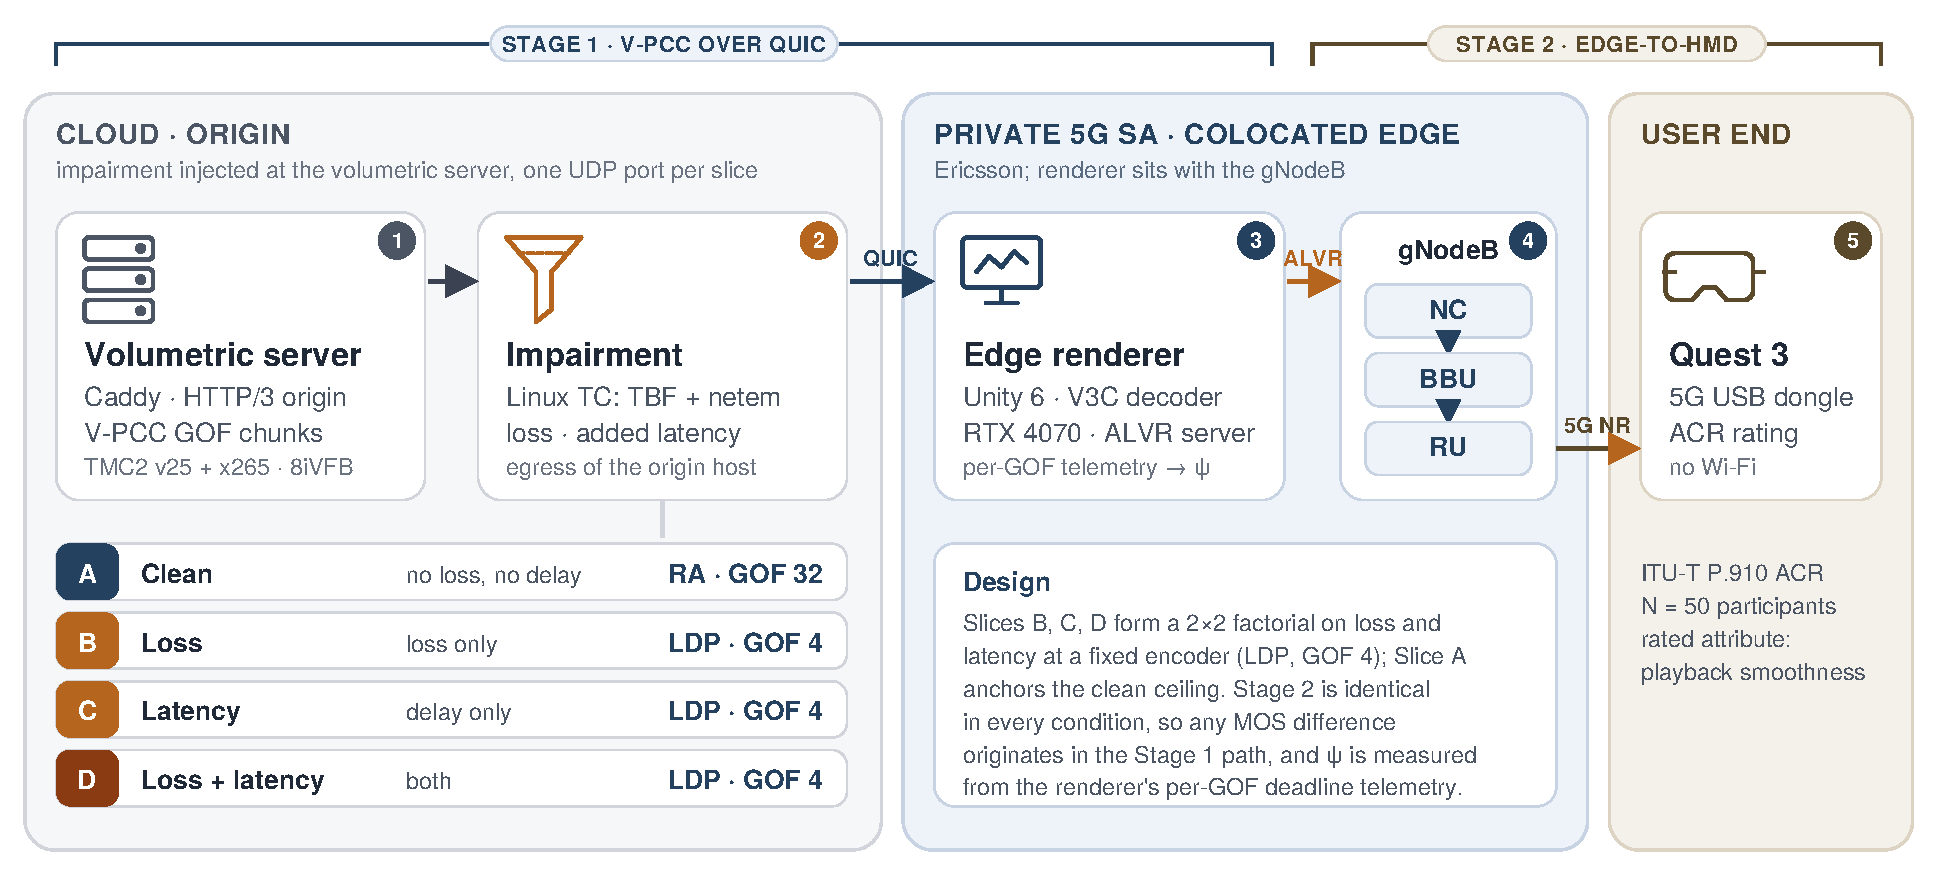
\includegraphics[width=\textwidth]{pipeline.pdf}
  \caption{End-to-end pipeline. Stage~1 delivers \vpcc content from the
  volumetric server~\ding{172}, where impairment is injected at the
  host's egress on one UDP port per slice~\ding{173}, over reliable
  \quic to the edge renderer~\ding{174}, colocated with the
  gNodeB~\ding{175} of the private \fiveg network. Stage~2 casts the
  rendered stereo frames through the network controller, baseband unit
  and radio unit to the Meta Quest~3~\ding{176} and is identical across
  conditions.}
  \label{fig:architecture}
\end{figure*}

\begin{table}[t]
  \caption{Testbed components.}
  \label{tab:testbed}
  \centering
  \small
  \begin{tabular}{@{}ll@{}}
    \toprule
    Component & Specification \\
    \midrule
    Volumetric server & Ubuntu 24.04, Caddy v2.11 (quic-go), HTTP/3, TLS~1.3 AES-128-GCM \\
    Impairment        & Linux TC (TBF + netem chain), one UDP port per slice \\
    Edge renderer     & Windows~11, NVIDIA RTX~4070, Unity~6, 5G-MAG V3C native decoder \\
    Presentation      & Native OpenGL$\to$DX11 interop plugin, SteamVR, ALVR \\
    5G network        & Ericsson private 5G SA, edge colocated with the gNodeB \\
    \hmd              & Meta Quest~3 (Snapdragon XR2 Gen~2), adapted 5G USB dongle \\
    \bottomrule
  \end{tabular}
\end{table}

\subsection{Content Preparation}
\label{sec:sys-content}

\paragraph{Sequences.}
Three sequences of the 8i Voxelized Full Bodies dataset~\cite{8i},
Category~2 of the \vpcc common test conditions~\cite{vpccctc}, are used
(Figure~\ref{fig:content}): Longdress (vox10, $\approx$0.85\,M
points/frame), Soldier (vox10, $\approx$1.08\,M) and ThaiDancer (vox12,
$\approx$3.13\,M). Each is \SI{10}{\second} long, 300 frames at
\SI{30}{fps}, and depicts a single person in motion.

\begin{figure}[t]
  \centering
  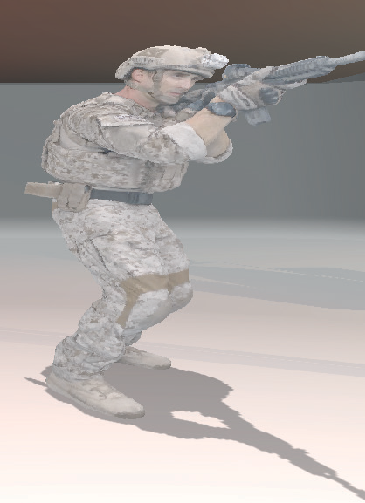
\includegraphics[height=2.6cm]{view-sd-front.pdf}\hfill
  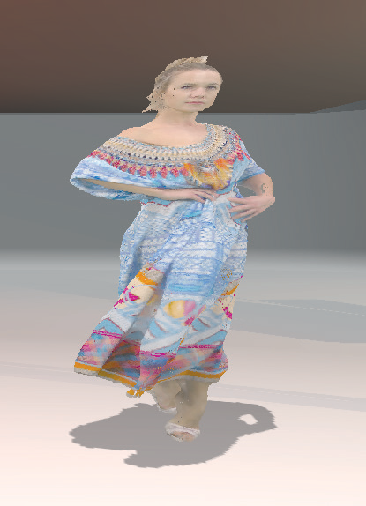
\includegraphics[height=2.6cm]{view-ld-front.pdf}\hfill
  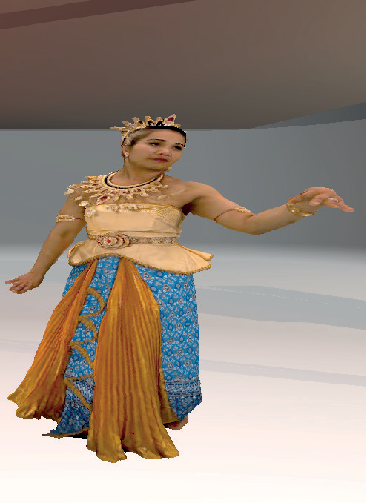
\includegraphics[height=2.6cm]{view-td-front.pdf}\hfill
  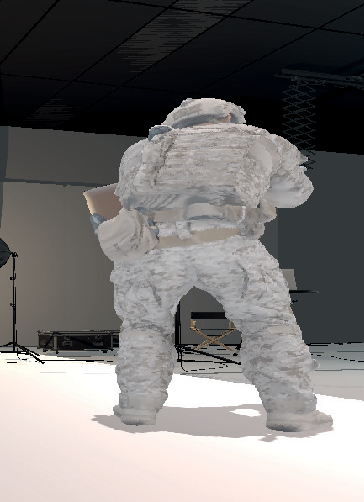
\includegraphics[height=2.6cm]{view-sd-back.pdf}\hfill
  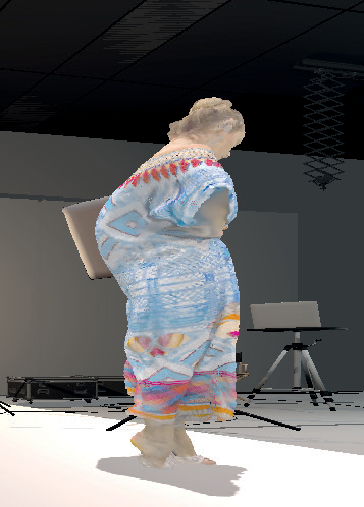
\includegraphics[height=2.6cm]{view-ld-back.pdf}\hfill
  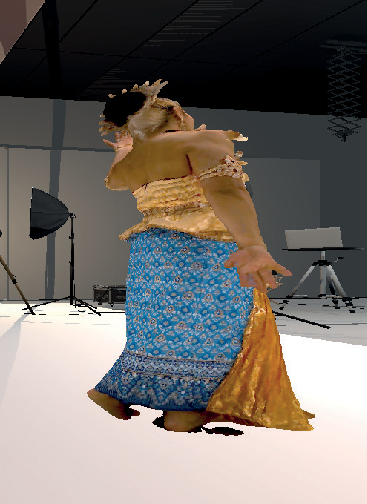
\includegraphics[height=2.6cm]{view-td-back.pdf}
  \caption{Soldier, Longdress and ThaiDancer in the rendering scene,
  front (first three) and back (last three) views.}
  \label{fig:content}
\end{figure}

\paragraph{Encoder.}
\gls{tmc2}~v25~\cite{tmc2} is the \vpcc reference software, but its
encoding time is dominated by the \gls{hevc} reference encoder
\gls{hm}, which codes the occupancy, geometry and attribute videos
separately. We replace \gls{hm} for the geometry and attribute videos
with x265~\cite{x265} through a command-line shim that accepts
\gls{hm}'s interface and dispatches FFmpeg~6.1 with libx265, so that
\gls{tmc2} runs unmodified and unaware of the substitution. The
\gls{ldp} configurations use \texttt{bframes=0},
\texttt{tune=zerolatency} and \texttt{preset=fast}; the \gls{ra}
configuration uses \texttt{bframes=15} and \texttt{preset=medium}.
Occupancy maps, which are coded losslessly, remain with \gls{hm}. With
the shim, one configuration of a vox10 sequence encodes in
\SIrange{25}{30}{\minute} and of the vox12 sequence in
\SIrange{110}{120}{\minute} on a single workstation, which makes a
multi-configuration sweep tractable.

The patch packer of \gls{tmc2} may change atlas dimensions within a
sequence, and the real-time decoder of Section~\ref{sec:sys-edge} does
not support such a change mid-stream. Atlas dimensions are therefore
fixed per sequence and configuration with \gls{tmc2}'s minimum image
width and height options (a minimum height of 4096 for ThaiDancer).

\paragraph{Encoding campaign.}
Each sequence is encoded in three configurations that differ in
prediction structure and \gof length: \gls{ra} with a hierarchical
I/P/B structure and a \gof of 32, as prescribed by the \vpcc common
test conditions~\cite{vpccctc}, and \gls{ldp} with I- and P-frames
only~\cite{hmctc} and \gofs of 16 and 4. Geometry QP (16) and occupancy
precision (2) are fixed and the attribute QP is swept.
Figure~\ref{fig:rd} reports the resulting rate--distortion curves of
the attribute video. Two observations guide the operating points. The
gap between sequences at a fixed bitrate (about \SI{4}{dB}) is an
order of magnitude larger than the gap between configurations of the
same sequence (\SIrange{0.3}{0.6}{dB}), so differences between contents
cannot be removed by encoder tuning; and \gls{ra} lies on or just
above the \gls{ldp} curves, so the shorter \gls{ldp} \gofs trade coding
efficiency for resilience to transport delay rather than for fidelity.
The attribute QPs selected (Table~\ref{tab:encoder}) give a
\gls{psnr}$_Y$ between 34 and \SI{39}{dB} and place all three sequences
in a common bitrate band (shaded), so that differences across
conditions are attributable to transport and content rather than to
bitrate. Attribute data dominate the bitstream: for Longdress,
attribute coding accounts for about 92\% of the encoded size, geometry
for 6\% and occupancy for 1\%. \pcqm~\cite{pcqm} is computed per
sequence as a stimulus descriptor and does not enter the model
(Section~\ref{sec:model-scope}).

\begin{figure}[t]
  \centering
  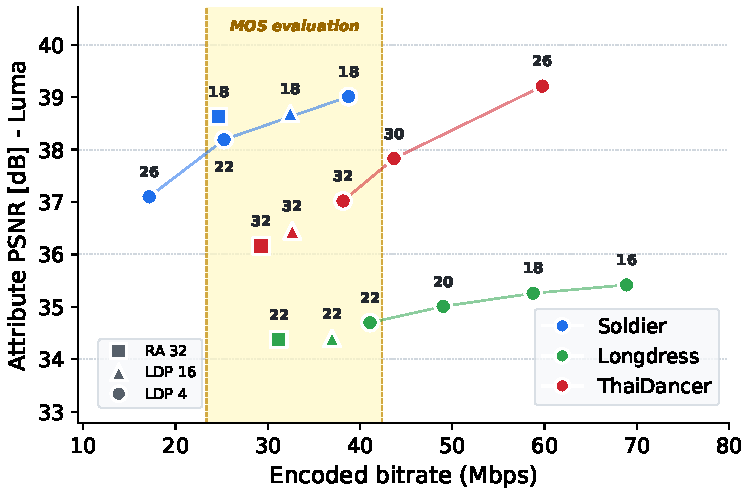
\includegraphics[width=0.62\linewidth]{rate-distortion.pdf}
  \caption{Rate--distortion curves of the attribute video for the three
  encoder configurations; labels are attribute QPs. The shaded band
  marks the bitrate range of the encoded sequences used in the
  subjective studies.}
  \label{fig:rd}
\end{figure}

\paragraph{Delivery units.}
Each bitstream is split into one object per \gof with the
VpccChunkCreator tool of the 5G-MAG platform~\cite{fivegmag}: a
300-frame sequence yields 75 objects of \SI{133}{\milli\second} at
\gls{ldp} \gof{}=4, 19 of \SI{533}{\milli\second} at \gls{ldp} \gof{}=16
and 10 of \SI{1067}{\milli\second} at \gls{ra} \gof{}=32. These objects
are the delivery units $k$ of Section~\ref{sec:model-layer1}.

\begin{table}[t]
  \caption{\vpcc encoder configuration.}
  \label{tab:encoder}
  \centering
  \small
  \begin{tabular}{@{}ll@{}}
    \toprule
    Parameter & Value \\
    \midrule
    Codec                          & MPEG TMC2 v25.0 \\
    HEVC (geometry / attribute)    & x265 3.5 (FFmpeg 6.1) via HM-compatible shim \\
    HEVC (occupancy, lossless)     & HM 16.20 + SCM 8.8 \\
    Geometry QP / occupancy precision & 16 / 2 (fixed) \\
    Attribute QP (Soldier / Longdress / ThaiDancer) & 18 / 22 / 32 \\
    Clean-reference profile        & \glsentryshort{ra}, \gof{}=32, I/P/B frames, 10 units \\
    Factorial profile              & \glsentryshort{ldp}, \gof{}=4, I/P frames, 75 units \\
    Structural contrast            & \glsentryshort{ldp}, \gof{}=16, I/P frames, 19 units \\
    \bottomrule
  \end{tabular}
\end{table}

\subsection{Origin, Transport and Impairment}
\label{sec:sys-stage1}

Volumetric video, like 2D video at scale, is delivered as time-bounded
HTTP objects: ISO/IEC 23090-10 packages \vpcc into ISOBMFF tracks and
\gls{dash} segments~\cite{v3ccarriage}, and the 5G-MAG platform plays
them from an HTTP origin~\cite{fivegmag}. The pipeline keeps this
object model but fetches each \gof over \gls{http3}. Over \gls{tcp}, a
lost segment blocks every byte behind it on the connection, so a loss
inside one \gof would also stall the next \gof in flight; \quic's
independent streams remove that coupling, and its combined
\gls{tls}~1.3 and transport handshake costs one round trip. It is also
the transport a deployed service would most plausibly use: in October
2026, 40.9\% of public web sites advertised
\gls{http3}~\cite{w3techs2026}.

The origin runs Caddy~v2 (quic-go) and serves each \gof object over
\gls{http3}. Objects leave the origin through a Linux Traffic Control
chain (TBF + netem) on the egress interface that implements the
impairment of each slice; each slice is bound to a distinct \gls{udp}
port, so all slices are served by one server instance without
cross-condition interference, and loss is accounted for exactly at the
IP layer. No partial-reliability or datagram extension is used, so the
transport behaviour is that of standard \quic~\cite{rfc9000}.

\subsection{Edge Decoding and Rendering}
\label{sec:sys-edge}

\paragraph{Fetching and decoding.}
The edge renderer is a Unity~6 application. Of the 5G-MAG \gls{v3c}
platform~\cite{fivegmag}, only the native decoder plugin, an optimised
\gls{tmc2} decoder, is used; its \gls{dash} client is replaced by an
\gls{http3} fetcher in the application. A paced controller keeps up to
three \gof requests in flight, issues each request
\SI{200}{\milli\second} ahead of the unit's presentation time and
assigns it a wall-clock deadline. A unit that misses its deadline is
substituted by the last good \gof, the hold-then-drop policy of
Section~\ref{sec:model-layer1} that turns late delivery into freezes
and frame skips. For every unit the renderer logs request time,
completion time, size and deadline outcome; this log is the input of
the Layer~1 analysis.

\paragraph{Presentation bridge.}
The decoder's synthesiser renders the reconstructed point cloud with
OpenGL, whereas the SteamVR compositor that feeds the casting stage
consumes DirectX~11 textures, and Unity's OpenXR path cannot hand the
decoder's OpenGL output to it. A native plugin bypasses that path: for
each eye it shares the OpenGL render target with a DirectX~11 texture
through the \texttt{WGL\_NV\_DX\_interop2} extension, a zero-copy
operation, and submits the texture to the compositor with OpenVR's
\texttt{IVRCompositor::Submit}. The point cloud is thus rendered once
per eye on the edge GPU with head-tracked \gls{6dof} viewing, and no
frame is copied through system memory.

\subsection{\fiveg Access for the Headset}
\label{sec:sys-stage2}

The edge renderer is colocated with the gNodeB of an Ericsson private
\fiveg standalone network, and ALVR casts the composited stereo frames
to the Meta Quest~3. Because the Quest~3 has no 5G modem, a commercial
5G USB dongle is adapted to its USB-C port and exposed to the headset
as a network interface, so the last hop traverses the 5G radio access
network rather than Wi-Fi~\cite{vquest2026}. Throughput on this link,
measured with on-device capture (PCAPdroid), is not a bottleneck for
the casting stream, and Stage~2 is held identical across all
conditions.

\section{Experimental Design}
\label{sec:design}

\subsection{Preliminary Three-Tier Study}
\label{sec:design-pilot}

The design builds on a three-tier study run on the same pipeline
($N=20$)~\cite{mosaic2026}. Each tier paired a network profile with
the encoder configuration an operator would deploy for it: a clean
tier (A) with \gls{ra} \gof{}=32; a loss-dominant tier (B, 1.9\% loss,
\SI{5}{\milli\second} added latency) with \gls{ldp} \gof{}=16; and a
latency-dominant tier (C, 0.6\% loss, \SI{9}{\milli\second}) with
\gls{ldp} \gof{}=4. The three sequences were rated in a fixed order on
the \gls{acr} scale. Figure~\ref{fig:pilot} summarises the outcome.
Mean opinion fell monotonically from 4.72 (A) to 4.07 (B) and 3.21
(C), with the strongest content dependence on Longdress
($4.89 \rightarrow 2.21$), the most attribute-dominated bitstream
(Section~\ref{sec:sys-content}). Tier~C carried \emph{less} loss than
tier~B yet scored lower, pointing to the \gof deadline budget rather
than loss magnitude as the driver. The per-session deadline-miss rate
correlated with the ratings only partially
($\rho_{\mathrm{Spearman}} = -0.34$, $p < 10^{-3}$), because a missed
unit removes a different duration of content at each \gof length. On
the transport side, goodput varied more across sequences
(\SIrange{33}{42}{Mbps}) than across tiers (under \SI{6}{Mbps} within a
sequence) and did not fall under impairment, as \quic's congestion
controller reclaimed throughput after each recovery.

\begin{figure}[t]
  \centering
  \begin{subfigure}[b]{0.49\linewidth}
    \centering
    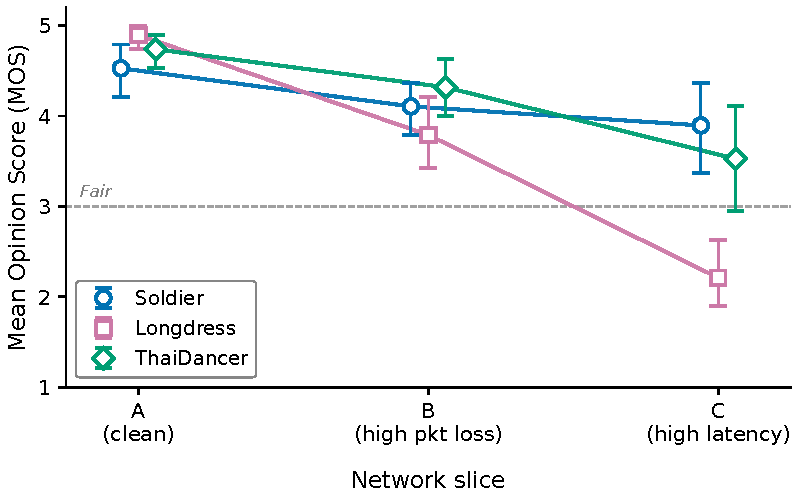
\includegraphics[width=\linewidth]{mosaic-mos.pdf}
    \caption{Mean opinion score with 95\% \gls{ci}.}
    \label{fig:pilot-mos}
  \end{subfigure}\hfill
  \begin{subfigure}[b]{0.49\linewidth}
    \centering
    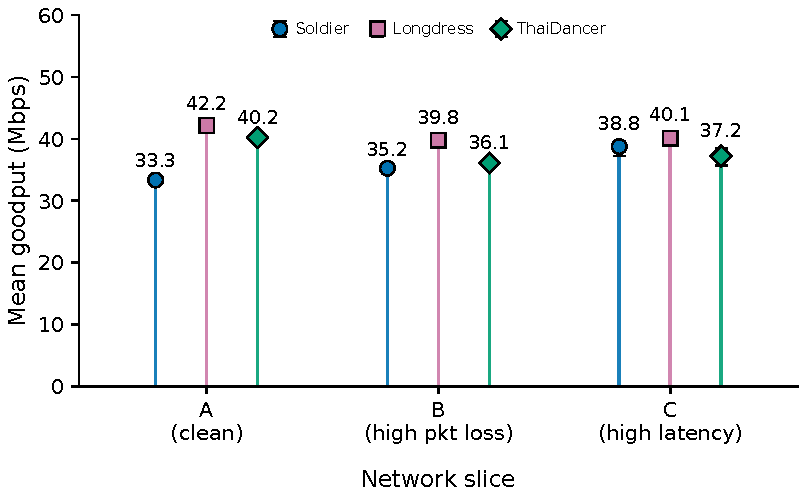
\includegraphics[width=\linewidth]{mosaic-goodput.pdf}
    \caption{Mean application-layer goodput.}
    \label{fig:pilot-goodput}
  \end{subfigure}
  \caption{Three-tier study ($N=20$), per sequence and tier; data
  from~\cite{mosaic2026}.}
  \label{fig:pilot}
\end{figure}

Four lessons shape the present design. Impairment and encoder
configuration were confounded in every tier, so the factorial slices
below hold the encoder fixed. The deadline-miss rate is an incomplete
predictor, so the analysis uses the temporal loss fraction $\tlf$,
which weights each miss by the content it removes. The presentation
order was fixed, so the present study balances it with a Latin square.
And goodput was not the limiting resource, so impairment is applied as
loss and added latency rather than as bandwidth caps.

\subsection{Network Conditions}
\label{sec:design-network}

Four slices share one origin and one renderer
and differ only in the impairment applied at the origin's egress
(Table~\ref{tab:impairments}). Slice~A is the clean reference: no
added loss or latency, \gls{ra} \gof{}=32, the profile an adaptive
service would choose on an unimpaired path, and the slice from which
the ceilings $\qc$ of Eq.~\eqref{eq:ceiling} and the slack $S_k$ of
Eq.~\eqref{eq:slack} are measured. Slices B, C and D form a $2\times2$
factorial on loss and added latency at a fixed encoder, \gls{ldp}
\gof{}=4: B applies loss only, C latency only, and D both at the same
levels, so that the single-factor effects and their combination are
estimated from the same stimuli. A fifth block, E, repeats the D
impairment at \gls{ldp} \gof{}=16 and provides the delivery-unit
contrast of Section~\ref{sec:model-layer1}; it is a separate rating
block rather than a factor, because its purpose is to test the
structural prediction at one operating point, not to map the
\gof\,$\times$\,impairment plane.

The impairment levels are chosen so that each factor alone produces a
measurable but not saturating effect: the loss rate and the added
one-way latency each sit inside the graded region established
in~\cite{mosaic2026}, where mean opinion stayed above the ``Fair''
threshold for most content, and are anchored to the 5G service
performance targets of~\cite{3gpp22261}. Loss is applied as random
(Bernoulli) loss by netem; latency as a fixed one-way delay without
jitter, so that the slack consumed by a unit is deterministic apart
from loss. Loss is accounted for at the IP layer of the origin, and
the renderer's telemetry records, for every unit, the request time,
completion time and deadline outcome, from which $\tlf$ is computed as
in Eq.~\eqref{eq:tlf}.

\begin{table}[t]
  \caption{Impairment slices. All slices share the same origin,
  renderer and casting stage; B--D hold the encoder fixed. \todo{fill
  $p$ and $\ell$}}
  \label{tab:impairments}
  \centering
  \small
  \begin{tabular}{@{}llllll@{}}
    \toprule
    Slice & Loss $p$ & Added latency $\ell$ & Encoder & Role & Rated by \\
    \midrule
    A & 0\%         & \SI{0}{\milli\second}        & \glsentryshort{ra}, \gof{}=32  & clean reference; $\qc$, $S_k$ & all \\
    B & \todo{$p$}  & \SI{0}{\milli\second}        & \glsentryshort{ldp}, \gof{}=4  & loss only & all \\
    C & 0\%         & \todo{$\ell$}                & \glsentryshort{ldp}, \gof{}=4  & latency only & all \\
    D & \todo{$p$}  & \todo{$\ell$}                & \glsentryshort{ldp}, \gof{}=4  & combined & all \\
    E & \todo{$p$}  & \todo{$\ell$}                & \glsentryshort{ldp}, \gof{}=16 & delivery-unit contrast & \todo{subset / all} \\
    \bottomrule
  \end{tabular}
\end{table}

\subsection{Subjective Experiment}
\label{sec:method}

\paragraph{Protocol.}
The study follows ITU-T P.910~\cite{p910} with the \gls{acr} method on
the five-point scale (5~Excellent to 1~Bad); a single-stimulus method
matches how a viewer consumes a stream and needs no reference
presentation inside the headset, unlike the double-stimulus methods of
ITU-R BT.500~\cite{bt500}. The rated attribute is
stated to participants as the \emph{smoothness of playback} of the
figure in front of them, not its visual fidelity; the instruction and
the training clips make the distinction explicit, because the
impairments under test manifest as freezes and frame skips while
spatial quality is fixed within a session
(Section~\ref{sec:model-scope}). Each stimulus is a
\SI{10}{\second} sequence played twice in a row (\SI{20}{\second}),
which exceeds the P.910 recommendation to leave time for \gls{6dof}
exploration without inducing fatigue~\cite{mosaic2026}. A session
opens with a training phase of about \SI{60}{\second} that shows the
three sequences on Slice~A so that the top of the scale is anchored
to the clean presentation, followed by the rated trials: three
sequences $\times$ four slices (A--D) for every participant, plus
block E, in a Latin-square order balanced across participants
so that no slice systematically follows another; this addresses the
fixed presentation order of~\cite{mosaic2026}. Ratings are given
verbally after each trial and entered by the experimenter, keeping
the participant's hands free and the headset on. A session lasts
about \SI{30}{\minute} including briefing and fitting.

\paragraph{Participants and screening.}
\todo{$N = 50$ participants (age range, gender split, prior \gls{vr}
experience), recruited from \anon[the institution]{UNICAMP} and
screened for normal or corrected-to-normal vision and absence of
discomfort during the training phase.} Participants rate in the
headset, standing, free to move within a \SI{2}{\metre} square;
head-tracked viewing is part of the stimulus and is not constrained.
Outlier screening follows ITU-T P.913~\cite{p913}: a participant whose
ratings deviate from the per-condition mean by more than the
prescribed bound in more than a quarter of conditions is excluded
before analysis.

\paragraph{Ethics.}
The protocol was approved by the institutional research ethics
committee through the national platform
(\anon[protocol number withheld for review]{Plataforma Brasil, CAAE
\todo{number}}); participants gave written informed consent, could
stop at any time, and were told they could remove the headset at the
first sign of discomfort. The study complies with the ACM policy on
research involving human participants.

\subsection{Data Processing and Statistical Analysis}
\label{sec:design-analysis}

\paragraph{Opinion scores.}
For each condition (sequence $\times$ slice) we report the mean
opinion score with a bootstrap 95\% \gls{ci} (10,000 resamples over
participants). Because \gls{acr} ratings are ordinal and the
per-condition distributions are not assumed normal, inference is
carried out with a \gls{clmm}: the rating is the ordinal response,
loss (present/absent) and latency (present/absent) are fixed effects
together with their interaction, and participant and sequence are
random intercepts. The two single-factor predictions of
Section~\ref{sec:model-predictions} correspond to the main effects;
the super-additivity prediction corresponds to a positive
loss$\times$latency interaction on the latent scale, and we also
report it on the \mos scale as the contrast
$(\mos_A - \mos_D) - (\mos_A - \mos_B) - (\mos_A - \mos_C)$ with its
bootstrap \gls{ci}. The delivery-unit prediction is the contrast
between blocks D and E at matched impairment.

\paragraph{Transport telemetry and $\tlf$.}
Every rated trial is aligned with the renderer's per-unit log for the
same session, from which the measured temporal loss fraction
$\tlf_{\mathrm{meas}}$ is computed as one minus the ratio of frames
rendered on schedule to frames due, Eq.~\eqref{eq:tlf}. The clean
slice supplies the per-unit slack $S_k$, the base round trip $\rho$
and the goodput $C$; the Layer~1 prediction $\tlf_{\mathrm{pred}}$ is
evaluated from Eqs.~\eqref{eq:recovery}--\eqref{eq:tlf} with the
slice's $(p, \ell)$ and the unit sizes $B_k$ of the bitstream, taking
the expectation over the loss count. Layer~1 is assessed by comparing
$\tlf_{\mathrm{pred}}$ with $\tlf_{\mathrm{meas}}$ per condition.

\paragraph{Model fitting and held-out evaluation.}
Layer~2 is fitted on \emph{measured} $\tlf$: with $\qc$ fixed by
Eq.~\eqref{eq:ceiling} from Slice~A, $\alpha$ is estimated by
non-linear least squares of Eq.~\eqref{eq:crystal} to the
per-condition \mos, and its 95\% \gls{ci} is obtained by bootstrap
over participants. Generalisation is tested by leave-one-out: $\alpha$
is refitted with one slice (or one sequence) withheld and the withheld
condition is predicted without refitting; we report \gls{plcc},
\gls{srocc} and \gls{rmse} on the withheld conditions, pooled. The same
protocol is applied to the five-coefficient regression of
Eq.~\eqref{eq:udora}, refitted on our ratings per sequence, so that
the comparison with the prior model is at equal data and equal
held-out protocol rather than against published figures.

\section{Results}
\label{sec:results}

\subsection{Transport Characterization}
\label{sec:res-transport}
\todo{Layer~1 checks against logs (Table~\ref{tab:predictions}):
pure-delay threshold versus the delay scan; $p_{\mathrm{slow}}$ of
Eq.~\eqref{eq:pslow} versus the logged slow-unit fraction per session,
with $r_0$ and $\kappa$ from the server logs; Monte Carlo $\tlf$ and
its between-session spread versus the logged $\tlf$; the regime
boundary versus the sessions that collapsed. Figure slot: measured
versus predicted $p_{\mathrm{slow}}$ and $\tlf$ per slice and
sequence.}

\subsection{Analysis of Opinion Scores}
\label{sec:res-mos}
\todo{Per-slice and per-sequence \mos with bootstrap \glspl{ci};
\gls{clmm} with slice as fixed effect; B, C and D versus A. Figure
slot: \mos per sequence and slice.}

\subsection{One Perceptual Channel}
\label{sec:res-channel}
\todo{Test of Claim~1: \mos versus measured $\tlf$ with all slices
and sequences on one axis; \gls{clmm} with $\tlf$ (and $\phi$) as
covariates and the likelihood-ratio test for slice identity; sessions
with $\tlf \approx 0$ on impaired slices versus Slice~A; the freeze
extension $\alpha_\phi = 0$. Figure slot: \mos versus $\tlf$ with the
\crystal curve overlaid.}

\subsection{Model Calibration and Held-out Prediction}
\label{sec:res-calibration}
\begin{table}[t]
  \caption{Fitted \crystal parameters with 95\% bootstrap \glspl{ci}.
  \todo{fill}}
  \label{tab:params}
  \centering
  \small
  \begin{tabular}{@{}lllll@{}}
    \toprule
    Quantity & Estimate & CI low & CI high & Note \\
    \midrule
    $\alpha$ (single, pooled)         & & & & $\tlf_{1/2} = \ln 2/\alpha$ \\
    $\alpha_\phi$ (freeze extension)  & & & & test of $\alpha_\phi = 0$ \\
    $\qc$ Soldier / Longdress / ThaiDancer & & & & from Slice~A \\
    Held-out \gls{plcc} / \gls{srocc} / \gls{rmse} & & & & vs.\ 0.57--0.66~\cite{udora2026tmm} \\
    \bottomrule
  \end{tabular}
\end{table}
\todo{$\alpha$ and its \gls{ci}; leave-one-slice-out and
leave-one-sequence-out prediction; Table~\ref{tab:params}.}

\subsection{Comparison with Prior Models}
\label{sec:res-comparison}
\todo{Held-out \gls{plcc}/\gls{srocc}/\gls{rmse} of \crystal against a
re-fit of Eq.~\eqref{eq:udora} and a separable model in $(d, P)$ on
the same ratings; parameter count versus accuracy.}

\section{Discussion}
\label{sec:discussion}

\subsection{Why One Parameter Suffices}
\todo{Interpret: the per-level coefficients of Eq.~\eqref{eq:udora}
absorb what $\tlf$ expresses; the interaction lives in the transport
layer, not in perception; what the fitted $\alpha$ and $\tlf_{1/2}$
mean for a viewer.}

\subsection{Implications for Private \fiveg Dimensioning}
\todo{Keep brief: the pure-delay threshold and the loss ladder at
\SI{9}{\milli\second} as operating envelopes; a full tutorial treatment
is out of scope.}

\subsection{Limitations}
\todo{Internal (emulation at the origin versus live radio impairment;
one client with $f$ and $H$ fixed), external (three contents, one
\hmd, one testbed), construct (\mos on smoothness versus task
performance); the effective recovery cost $r(d)$ as a per-unit
approximation of a process with memory.}

\subsection{Extension to Other Representations}
\label{sec:model-predict}
\todo{Layer~1 with $G = 1$ (no delivery-unit coupling): Udora et al.'s
uncompressed per-frame streaming and the frame-independent delivery
of~\cite{vquest2026} as external checks.} 3D Gaussian
Splatting~\cite{kerbl2023gaussian} is acquiring a streaming literature
of its own~\cite{sun2025lts}, evaluated with objective rendering
metrics. Because each Gaussian primitive is independently decodable, a
splat stream has no \gof coupling in the sense of
Section~\ref{sec:model-unit}. \todo{State what Layer~1 predicts for
\threedgs and what observation would falsify it.}

\section{Conclusion and Future Work}
\label{sec:conclusion}
\todo{Restate Claim~1 and its support; the pipeline as a reusable
instrument.} Two predictions of Layer~1 remain untested here. The
budget $B_{\mathrm{eff}}$ and the slack $S$ grow with the \gof size
$G$ while the per-loss cost $r(d)$ does not, so a longer low-delay
\gof should absorb more losses per unit and be more resilient at
matched impairment than a shorter one, against the intuition that
shorter units limit damage; the three-tier study pointed the same
way~\cite{mosaic2026}, and a rated \gls{ldp} \gof{}=16 block at the
levels of Table~\ref{tab:impairments} would test it. And a
representation without delivery-unit coupling, such as per-frame
point clouds or Gaussian splats, should show no interaction between
delay and loss. \todo{Live radio impairment rather than emulation;
adaptive-profile (\gls{ra} \gof{}=32) evaluation.}


%% ------------------------------------------------------------------
\begin{acks}
\anon[Acknowledgments withheld for review.]{%
This work was supported by the FAPESP Engineering Research Center
SMARTNESS (Proc.\ 2021/00199-8). \todo{Add CAPES/CNPq/Ericsson
acknowledgments as applicable.}
}
\end{acks}

\bibliographystyle{ACM-Reference-Format}
\bibliography{references}

%% Online Appendix. Toggle \appendixtrue / \appendixfalse in the preamble
%% (switched off while checking the body's page count).
\ifappendix
\clearpage
\appendix
\renewcommand{\topfraction}{0.95}\renewcommand{\bottomfraction}{0.95}
\renewcommand{\textfraction}{0.05}\renewcommand{\floatpagefraction}{0.8}
\setcounter{totalnumber}{4}\setcounter{topnumber}{3}
\section{Subjective Study Materials}
\label{app:study}
\todo{Session script, rating interface screenshot, exact slice ordering.}

\section{Supplementary Fit Diagnostics}
\label{app:fits}
\todo{Residual plots, alternative model forms considered (additive,
logistic) and why they were rejected.}

\fi

\end{document}
